%*****************************************
\chapter{Lab 04: Descriptives]}\label{ch:lab04}
%*****************************************
%\setcounter{figure}{10}
%\NoCaseChange{Homo Sapiens}

\section{Introduction}

It is typical for a researcher to report a number of descriptive attributes of a dataset, like its mean or standard deviation and this lab describes how to generate that sort of statistical analysis.

\section{Discussion}

\subsection{Descriptive Measures}

The descriptive measures commonly reported are\footnote{These measures are described in \nameref{ch:lab03} on page \ref{ch:lab03}.}:

\begin{itemize}
  \item Kurtosis
  \item Mean
  \item Maximum Value
  \item Minimum Value
  \item Range
  \item Skewness
  \item Standard Deviation
  \item Standard Error
  \item Sum
  \item Variance
\end{itemize}

\subsection{Z-Scores}\label{z-scores}

A Z-Score is how many standard deviations\footnote{Standard Deviation is described on page \pageref{lab03_standard_deviation}} a data point lies above or below the mean. In other words, a Z-Score re-scales, or standardizes, the data points so they can be more easily compared. Here are a few facts about Z-Scores:

\begin{itemize}
  \item A z-score equal to $ 0 $ is a data point that is equal to the mean.
  \item A z-score less than $ 0 $ is a data point that is less than the mean.
  \item A z-score greater than $ 0 $ is a data point that is greater than the mean.
  \item A z-score equal to $ +1 $ is a data point that is $ 1 $ standard deviation greater than the mean.
  \item A z-score equal to $ -1 $ is a data point that is $ 1 $ standard deviation less than the mean.
\end{itemize}

For example, imagine that a student took an exam and scored $ 15 $. Is the a good score? It would depend on the mean and standard deviation for that exam. The easiest way to check is to convert the student's score of $ 15 $ to a Z-Score, which accounts for both mean and standard deviation. If a score of $ 15 $ is converted to a Z-Score of $ +1 $ then the student scored higher than about $ 68\% $ of the other students so that would be a good score.

Z-Scores can also be used to compare the results of two tests where the mean and standard deviation may be different. For example, imagine that a state changes the annual test that is given to fourth, sixth, and ninth graders. A particular student scored $ 40 $ on the math portion in the fourth grade and then scored $ 30 $ on the new text in the sixth grade. That would not necessary mean that the student is doing worse because the test may be harder. In order to compare those two test results a researcher would have to know the mean and standard deviation of the two tests. Again, converting the student's scores to Z-Scores would help determine whether the student is making progress. Imagine that for the fourth grade exam the student's Z-Score is $ -0.3 $, or slightly below the mean, but on the sixth grade test the student's Z-Score is $ +0.3 $, or slightly above the mean. Even though the raw scores seem to show a decrease in score the Z-Score reveals that the student is making above normal progress.

Calculating Z-Scores is a simple formula:
 
\begin{center}
  $ Z = \frac{X - mean}{SD} $
\end{center}

Where \textit{X} is a specific data point and \textit{SD} is the standard deviation of the dataset. Thus, if a dataset has a mean of $ 50 $ and a standard deviation of $ 10 $ then the data point $ 55 $ has a Z-Score of $ +0.5 $:

\begin{center}
  $ +0.5 = \frac{55 - 50}{10} $
\end{center}

\section{Procedure}

\subsection{Descriptives}

Start \acs{PSPP} and open the \textit{bdims} dataset, then:

\begin{enumerate}
  \item Click \textsc{\fbox{Analyze $ \rightarrow $ Descriptive Statistics $ \rightarrow $ Descriptives}}
  \item Click the phrase \textit{navel (abdominal) girth} in the left column and then click the right-arrow button near the center of the window to move it to the ``Variables'' box on the right side of the window. (Alternatively, double-click the phrase \textit{navel (abdominal) girth} in the left column to move it to the ``Variables'' box.) NOTE: This is displayed as ``nav.gi'' in the ``Variables'' box since that is the actual name of the variable.
  \item Check the following ``Statistics'' options in the lower-right box: Mean, Standard Deviation, Minimum, and Maximum.
  \item Uncheck all options at the bottom of the window.
  \item Click \fbox{OK} to generate the descriptives.
\end{enumerate}

\begin{figure}[H]
  \begin{center}
    \fbox{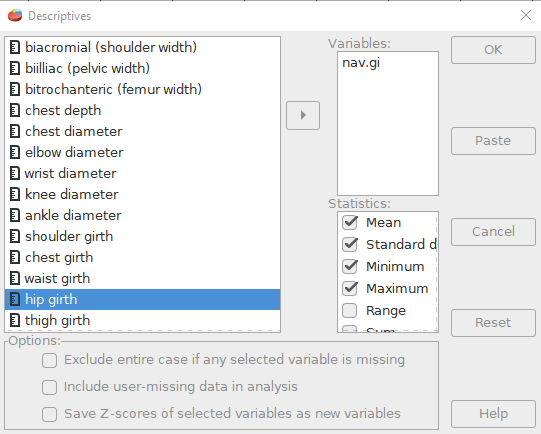
\includegraphics[width=\linewidth]{gfx/lab04_fig01}}
    \caption{Generating Descriptives}
    \label{lab04_fig01}
  \end{center}
\end{figure}

\begin{figure}[H]
  \begin{center}
    \fbox{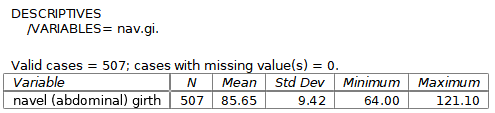
\includegraphics[width=\linewidth]{gfx/lab04_fig02}}
    \caption{Navel Girth Descriptives}
    \label{lab04_fig02}    
  \end{center}
\end{figure}

\subsubsection{Activity 1: Descriptives} \label{lab04_act01}

Using the \textit{bdims} dataset, produce the descriptives for \textit{age}. Include the mean, standard deviation, minimum, and maximum statistics.

\subsubsection{Activity 2: Descriptives} \label{lab04_act02}

Using the \textit{cafe} dataset, produce the descriptives for \textit{age}. Include the mean, standard deviation, minimum, and maximum statistics.

\subsection{Z-Scores}

Start \acs{PSPP} and open the \textit{gifted} dataset, then:

\begin{enumerate}
  \item Click \textsc{\fbox{Analyze $ \rightarrow $ Descriptive Statistics $ \rightarrow $ Descriptives}}
  \item Click the word \textit{motherIQ} in the left column and then click the right-arrow button near the center of the window to move it to the ``Variables'' box on the right side of the window. (Alternatively, double-click the word \textit{motherIQ} in the left column to move it to the ``Variables'' box.)
  \item Check the following ``Statistics'' options in the lower-right box: Mean, Standard Deviation, Minimum, and Maximum.
  \item Check the ``Save Z-scores of selected variables as new variables'' option at the bottom of the window.
  \item Click \fbox{OK} to generate the descriptives.
\end{enumerate}

\begin{figure}[H]
  \begin{center}
    \fbox{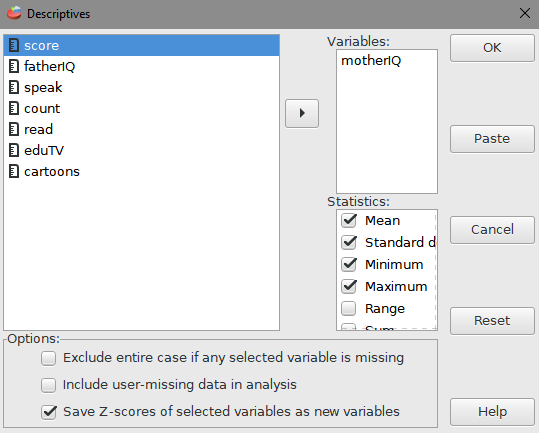
\includegraphics[width=\linewidth]{gfx/lab04_fig03}}
    \caption{Generating Descriptives}
    \label{lab04_fig03}
  \end{center}
\end{figure}

\begin{figure}[H]
  \begin{center}
    \fbox{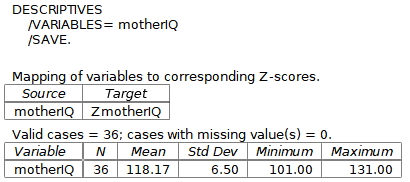
\includegraphics[width=\linewidth]{gfx/lab04_fig04}}
    \caption{Descriptives for Mother's IQ}
    \label{lab04_fig04}
  \end{center}
\end{figure}

After the Descriptives are generated the Z-Scores for Mother's IQ are calculated and added to a new field in the dataset.

\begin{figure}[H]
  \begin{center}
    \fbox{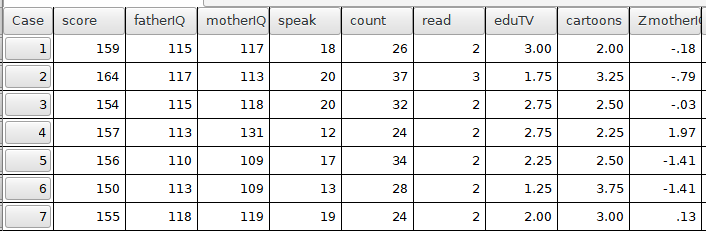
\includegraphics[width=\linewidth]{gfx/lab04_fig05}}
    \caption{Z-Scores for Mother's IQ}
    \label{lab04_fig05}
  \end{center}
\end{figure}

The Z-Scores are in the last column on the right. For example, case one has Mother's IQ of $ 117 $ and Z-Score of $ -0.18 $ which is slightly below the mean for this dataset. Case four, on the other hand, has Mother's IQ of $ 131 $ and Z-Score of $ +1.97 $, which is significantly above the mean for this dataset.

\subsubsection{Activity 3: Z-Scores} \label{lab04_act03}

Using the \textit{gifted} dataset, produce the Z-Scores for \textit{speak}. Report the Z-Score for any case where the ``speak'' raw score is $ 18 $. 

\subsubsection{Activity 4: Z-Scores} \label{lab04_act04}

Using the \textit{cafe} dataset, produce the Z-Scores for \textit{age}. Report the Z-Score for any case where the ``age'' raw score is $ 30 $. 

\section{Deliverable}

Complete the following activities in this lab:

\rowcolors{1}{gray!25}{}
\begin{center}
  \begin{tabular}{lll}
    \hline 
    \textbf{Number} & \textbf{Name} & \textbf{Page} \\ 
    \hline 
    \ref{lab04_act01} & \nameref{lab04_act01} & \pageref{lab04_act01} \\ 
    \ref{lab04_act02} & \nameref{lab04_act02} & \pageref{lab04_act02} \\ 
    \ref{lab04_act03} & \nameref{lab04_act03} & \pageref{lab04_act03} \\ 
    \ref{lab04_act04} & \nameref{lab04_act04} & \pageref{lab04_act04} \\ 
    \hline 
  \end{tabular} 
\end{center}

Consolidate the responses for all activities into a single document and submit that document for grading.


